\section{GridDatamining}

\begin{frame}
	\frametitle{Data Mining: Objectives}
		\begin{itemize}
			\item<1-> {Estimate runtime in 'constant' time}
				\begin{itemize}
					\item<2-> {Constant to the amount of tasks already executed}	
				\end{itemize}
				\item<3-> {Estimation based on variable amounts of parameters}
			\end{itemize}
\end{frame}		
		
\begin{frame} 
	\frametitle{Data Mining: Concepts}
		\begin{itemize}
			\item<1-> {Strong correlation between parameters and runtime of a task}
			\item<2-> {Tasks with similar parameters have similar runtime}
				\begin{itemize}
					\item<3-> {Tasks with identical parameters have identical runtime}	
				\end{itemize}	
		\end{itemize}
\end{frame}


\begin{frame}
	\frametitle{Grid Data Mining: Basic Design}
	\begin{minipage}[t]{0.42\linewidth}
		\begin{itemize}
			\item<1-> {Array of 'grid points'}
				\begin{itemize}
					\item<2-> {Similar to a Cartesian coordinate system}
					%\item<3->{grid points: "pointer" to 'closest' task already executed}
					%\begin{itemize}
					%	\item<4->{closest defined as 'smallest parameter differences'}	
					%\end{itemize}
				\end{itemize}	
		\end{itemize}
	\end{minipage}\hfill
	\begin{minipage}[t]{0.58\linewidth}
		\vspace{-\ht\strutbox}
	\begin{tikzpicture}[scale = 0.5]
		\draw[->, very thick] (0,0) -- (7, 0) node[right] {param 1};
		\draw[->, very thick] (0,0) -- (0, 8) node[above] {param 2};
		
		\fill (1, 2) circle (0.5mm);
		\fill (2, 2) circle (0.5mm);
		\fill (3, 2) circle (0.5mm);
		\fill (4, 2) circle (0.5mm);
		\fill (5, 2) circle (0.5mm);
	
		\fill (1, 3) circle (0.5mm);
		\fill (2, 3) circle (0.5mm);
		\fill (3, 3) circle (0.5mm);
		\fill (4, 3) circle (0.5mm);
		\fill (5, 3) circle (0.5mm);
	
		\fill (1, 4) circle (0.5mm);
		\fill (2, 4) circle (0.5mm);
		\fill (3, 4) circle (0.5mm);
		\fill (4, 4) circle (0.5mm);
		\fill (5, 4) circle (0.5mm);
		
		\fill (1, 5) circle (0.5mm);
		\fill (2, 5) circle (0.5mm);
		\fill (3, 5) circle (0.5mm);
		\fill (4, 5) circle (0.5mm);
		\fill (5, 5) circle (0.5mm);
		
		\fill (1, 6) circle (0.5mm);
		\fill (2, 6) circle (0.5mm);
		\fill (3, 6) circle (0.5mm);
		\fill (4, 6) circle (0.5mm);
		\fill (5, 6) circle (0.5mm);
		
		\begin{scope}[>= Latex]
			\draw[->, very thick] (6, 6) node[right]{grid point}  --  (5.05, 6) ;
		\end{scope}
	\end{tikzpicture}
	\end{minipage}		
\end{frame}

\begin{frame}
	\frametitle{Grid Data Mining: Basic Design}
	\begin{minipage}[t]{0.48\linewidth}
		%\begin{itemize}
		%	\item<1-> {Array of 'grid points'}
				\begin{itemize}
		%			\item<2-> {Similar to a Cartesian coordinate system}
					\item<1->{grid points: "pointer" to 'closest' task already executed}
					\begin{itemize}
						\item<2->{closest defined as 'smallest parameter differences'}	
					\end{itemize}
				\end{itemize}	
		%\end{itemize}
	\end{minipage}\hfill
	\begin{minipage}[t]{0.48\linewidth}
		\vspace{-\ht\strutbox}
	\begin{tikzpicture}[scale = 0.8]
	%\fill[white] (-2, 6) circle (0.01);
	
		\fill (1, 2) circle (0.5mm);
		\fill (5, 2) circle (0.5mm);
		\fill (1, 6) circle (0.5mm);
		\fill (5, 6) circle (0.5mm);
		
		\fill[green!75!black] (2, 2) circle (0.5mm);
		\fill[green!75!black] (7, 3) circle (0.5mm);
		\fill[green!75!black] (2, 5) circle (0.5mm);
		\fill[green!75!black] (7, 4) circle (0.5mm);
				
		\draw[->] (1, 2) -- (1.95, 2);
		\draw[->] (5, 2) -- (6.97, 2.97);
		\draw[->] (1, 6) -- (1.97, 5.03);
		\draw[->] (5, 6) -- (6.97, 4.03);		
		
		\begin{scope}[>= Latex]
			\draw[->] (6, 4) node[left]{previous task}  --  (6.95, 4) ;
			\draw[->] (4, 6) node[left]{grid point}  --  (4.95, 6) ;
		\end{scope}
	\end{tikzpicture}
	\end{minipage}		
\end{frame}

\begin{frame}
	\frametitle{Grid Data Mining: Design Details}
	\begin{minipage}[t]{0.45\linewidth}
		\begin{itemize}
			\item<1-> {Grid origin $\neq$ Cartesian origin}
			\item<2-> {Grid origin = grid point with the  smallest coordinates} 
			\item<3-> {Distance between two grid points in every dimension flexible}
				\begin{itemize}
					\item {'increment' vector consisting of all 'increment' values}	
				\end{itemize}
		\end{itemize}
	\end{minipage}\hfill
	\begin{minipage}[t]{0.55\linewidth}
		\vspace{-\ht\strutbox}
		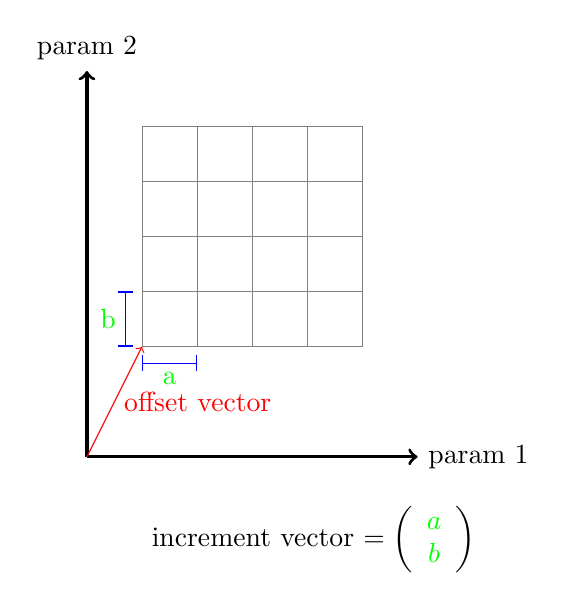
\begin{tikzpicture}[scale = 0.7]
		\draw[->, very thick] (0,0) -- (6, 0) node[right] {param 1};
		\draw[->, very thick] (0,0) -- (0, 7) node[above] {param 2};
		
		\draw[->, red] (0,0) -- node[right] {offset vector} (1, 2);
		
		\draw[step=1cm,gray,very thin] (1, 2) grid (5, 6);
		\draw[gray,very thin] (1, 2) -- (5, 2);
		\draw[gray,very thin] (1, 2) -- (1, 6);
		
		\draw (1, -1.5) node[right]{increment vector  $ = \left(\begin{array}{c} \textcolor{green}{a} \\ \textcolor{green}{b} \end{array}\right) \qquad$} ;
		
		 \draw[|-|, blue] (1, 1.7) -- node[below]{\textcolor{green}{a}} (2, 1.7);
		 \draw[|-|, blue] (0.7, 2) -- node[left]{\textcolor{green}{b}} (0.7, 3);
	\end{tikzpicture}
	\end{minipage}
\end{frame}

\begin{frame}
	\frametitle{Grid Data Mining: Runtime Approximation I}
	\begin{minipage}[t]{0.40\linewidth}
		\begin{itemize}
			\item<1->{Determine the surrounding grid points to a task}
			%\item<2->{Calculate the influence factor $F_i$ per grid point}
			%\begin{itemize}
				%\item<3->{Check whether the distance to the point is 0}
				%\begin{itemize}
				%	\item<4->{ $\Rightarrow$ influence factor $F_i$ is 1 $($ 													$\widehat{=}$ 100$\%$ influence$)$}
				%\end{itemize}
				%\item<5->{Otherwise calculate $F_i$ $($'Kastrati' value $F_i$ for grid 										point i$)$}
				%\begin{itemize}
			%		\item<3->{$d_i = \frac{D_i}{\Sigma D_i}$ $\widehat{=}$ relative distance}
					%\item<4->{$d_i \widehat{=}$ relative distance to grid point i}
					%\item<7->{$D_i \widehat{=}$ absolute distance to grid point i}
					%\item<4->{$\Sigma D_i \widehat{=}$ total distance to all 													surrounding grid points}
			%\end{itemize}
			%		\item<4->{$F_i = \frac{1}{\frac{d_i}{d_0} + \frac{d_i}{d_1} + ... + 										\frac{d_i}{d_n}}$}
				%\end{itemize}
		\end{itemize}
	\end{minipage}\hfill
	\begin{minipage}[t]{0.60\linewidth}
	\vspace{-\ht\strutbox}
		\begin{tikzpicture}
	%\fill[white] (-2, 6) circle (0.01);
	
		\fill (1, 2) circle (0.5mm);
		\fill (5, 2) circle (0.5mm);
		\fill (1, 6) circle (0.5mm);
		\fill (5, 6) circle (0.5mm);
		
		\fill[green!75!black] (2, 2) circle (0.5mm) node[above]{$T_0$};
		\fill[green!75!black] (7, 3) circle (0.5mm) node[right]{$T_1$};
		\fill[green!75!black] (2, 5) circle (0.5mm) node[above]{$T_3$};
		\fill[green!75!black] (7, 4) circle (0.5mm) node[right]{$T_2$};
				
		\draw[->] (1, 2) -- (1.95, 2);
		\draw[->] (5, 2) -- (6.97, 2.97);
		\draw[->] (1, 6) -- (1.97, 5.03);
		\draw[->] (5, 6) -- (6.97, 4.03);		
		
		\fill[red] (5, 3) circle (0.5mm);
		
		\begin{scope}[>= Latex]
			\draw[->] (4, 3) node[left]{appearing task}  --  (4.95, 3) ;
		\end{scope}
	\end{tikzpicture}
	\end{minipage}\hfill
\end{frame}

\begin{frame}
	\frametitle{Grid Data Mining: Runtime Approximation II}
	\begin{minipage}[t]{0.40\linewidth}
		\begin{itemize}
			%\item<1->{Determine the surrounding grid points to a task}
			\item<1->{Calculate the influence factor $F_i$ per grid point}
			%\begin{itemize}
				%\item<3->{Check whether the distance to the point is 0}
				%\begin{itemize}
				%	\item<4->{ $\Rightarrow$ influence factor $F_i$ is 1 $($ 													$\widehat{=}$ 100$\%$ influence$)$}
				%\end{itemize}
				%\item<5->{Otherwise calculate $F_i$ $($'Kastrati' value $F_i$ for grid 										point i$)$}
				%\begin{itemize}
					\item<3->{$d_i = \frac{D_i}{\Sigma D_i}$}
					%\item<4->{$d_i \widehat{=}$ relative distance to grid point i}
					%\item<7->{$D_i \widehat{=}$ absolute distance to grid point i}
					%\item<4->{$\Sigma D_i \widehat{=}$ total distance to all 													surrounding grid points}
			%\end{itemize}
					\item<4->{$F_i = \frac{1}{\frac{d_i}{d_0} + \frac{d_i}{d_1} + ... + 										\frac{d_i}{d_n}}$}
				%\end{itemize}
		\end{itemize}
	\end{minipage}\hfill
	\begin{minipage}[t]{0.60\linewidth}
	\vspace{-\ht\strutbox}
		\begin{tikzpicture}
	%\fill[white] (-2, 6) circle (0.01);
	
		\fill (1, 2) circle (0.5mm);
		\fill (5, 2) circle (0.5mm);
		\fill (1, 6) circle (0.5mm);
		\fill (5, 6) circle (0.5mm);
		
		\draw[->] (1, 2) -- (1.95, 2);
		\draw[->] (5, 2) -- (6.97, 2.97);
		\draw[->] (1, 6) -- (1.97, 5.03);
		\draw[->] (5, 6) -- (6.97, 4.03);
		
		%\fill[white] (1, 2) circle (0.5mm);
		%\fill[white] (5, 2) circle (0.5mm);
		%\fill[white] (1, 6) circle (0.5mm);
		%\fill[white] (5, 6) circle (0.5mm);
		
		\fill[green!75!black] (2, 2) circle (0.5mm) node[above]{$T_0$};
		\fill[green!75!black] (7, 3) circle (0.5mm) node[right]{$T_1$};
		\fill[green!75!black] (2, 5) circle (0.5mm) node[above]{$T_3$};
		\fill[green!75!black] (7, 4) circle (0.5mm) node[right]{$T_2$};
		
		\begin{scope}[>= Latex]
			\draw[<->, blue] (4.97, 2.99) -- node[below]{$D_0$} (2.03, 2.01);
			\draw[<->, blue] (5.05, 3) -- node[below]{$D_1$} (6.95, 3);
			\draw[<->, blue] (4.97, 3.02) -- node[above]{$D_3$} (2.03, 4.98);
			\draw[<->, blue] (5.02, 3.01) -- node[above]{$D_2$} (6.96, 3.98);
		\end{scope}
		
		\fill[red] (5, 3) circle (0.5mm);
	\end{tikzpicture}
	\end{minipage}\hfill
\end{frame}

\begin{frame}
	\frametitle {Grid Data Mining: Runtime Approximation III}	
		\begin{itemize}
			\item<1->{The total sum of all 'Kastrati' factors is 1}
			\item<2->{$\sum t_i * F_i$}
			\item<3->{$t_i$ = runtime of grid point i}					
			\item<4->{Multiply the runtime of each grid point with its corresponding 								factor}
		\end{itemize}				
\end{frame}

\begin{frame}
	\frametitle{Grid Data Mining: Task Insertion}
		\begin{itemize}
			\item<1->{Check whether the task is 'suited' as value of a 													surrounding grid point}
			\begin{itemize}
				\item<2->{Grid points 'always' contain the value of the 													closest task inserted to them}
				\item<3->{Note that inserting a point only adapts the 														closest grid points}
			\end{itemize}
			\item<4->{Adapts surrounding grid points, if necessary}
		\end{itemize}
		
		\begin{itemize}
			\item<5->{'Hard insert': checks ALL grid points and eventually adapts them}
		\end{itemize}	
\end{frame}

\begin{frame}
	\frametitle{Grid Data Mining: Evaluation}
		\begin{itemize}
			\item<1-> {Grid Data is evaluated on every insert}
			\item<2-> {Calculate average deviation}
			\item<3-> {Compare with set threshold}
			\begin{itemize}
				\item<4->{If higher: recreate grid}
			\end{itemize}
		\end{itemize}
\end{frame}	
	
\begin{frame}
	\frametitle{Grid Data Mining: Creation}
		\begin{itemize}
			\item<1-> {Initialize offset vector}
			\begin{itemize}
				\item<2-> {first creation: 0}
				\item<3-> {later: smallest value}
			\end{itemize}
			\item<4-> {Initialize increment vector}
			\begin{itemize}
				\item<5->{first creation: 1}
				\item<6->{later: 'data size' divided by number of fields}
			\end{itemize}
			\item<7-> {'Hard Insert' all tasks stored in database}			
		\end{itemize}
\end{frame}

%										☺
%\begin{frame}
%	\frametitle{}
%\end{frame}